\documentclass[11pt]{article}

\usepackage{fancyhdr}
\usepackage[margin=1in]{geometry}
\usepackage{xcolor,colortbl}
\usepackage[labelfont=bf,font=small]{caption}


\usepackage[T1]{fontenc}

\usepackage{enumitem}
\usepackage{todonotes}
\usepackage{titlesec}
\usepackage{tabularx}
\usepackage{parskip}
\usepackage{hyperref}
\usepackage{wrapfig}
\titlespacing\section{0pt}{0pt plus 4pt minus 2pt}{0pt plus 2pt minus 2pt}
\titlespacing\subsection{0pt}{12pt plus 4pt minus 2pt}{0pt plus 2pt minus 2pt}
\titlespacing\subsubsection{0pt}{12pt plus 4pt minus 2pt}{0pt plus 2pt minus 2pt}

\definecolor{Gray}{gray}{0.85}
\pagestyle{fancy}
\rfoot{\thepage}
\lfoot{\textbf{Research Statement} | D.A. Szafir}
\cfoot{}
\renewcommand{\headrulewidth}{0pt}
\renewcommand{\footrulewidth}{0.5pt}

%opening


\begin{document}
\setlength{\belowcaptionskip}{-10pt}
%\maketitle

\thispagestyle{fancy}

\textbf{\Large Research Statement}
{\hspace{220pt}\emph{Danielle Albers Szafir} \vspace{3pt}}
\hrule
%\\
%	{ 
%	\begin{tabularx}{\textwidth}{X X}
%		Assistant Professor & 315 UCB\\ 
%		Department of Information Science & University of Colorado Boulder \\ 
%		College of Media, Communication, \& Information &  Boulder, CO, 80309\\
%		University of Colorado Boulder & danielle.szafir@colorado.edu | 303.492.8532 
%	\end{tabularx}}}
%\hrule

%My research fuses methods from computer science, vision science, and cognitive science to model visual perception in order to develop novel visualization systems which support accurate analysis of complex data at unprecedented scales. These systems provide new analytics solutions in domains ranging from biology to the humanities. Through this work, I expand knowledge of visualization design by considering how the ubiquity and scales of data analysis fundamentally shift the demands placed on analytics tools.  %\vspace{-2pt}

Traditionally, visualizations have relied on perceptual models from psychology to communicate relationships in data.  However, these models ignore the complexities arising in real-world analytics applications, such as imperfect displays and crowded data distributions. These oversimplifications can cause people to misinterpret their data, leading to flawed understandings and erroneous conclusions. Further, current visualization approaches seldom blend visualization with other techniques, such as statistical analysis and machine learning or novel displays like augmented reality. However, combining effective visualization tools with novel computational and display technologies has the potential to greatly increase the accessibility and pervasiveness of data-driven reasoning. My research fuses methods from computer science, vision science, and cognitive science to model visual perception in order to develop novel visualization systems which support accurate analysis of complex data at unprecedented scales.

My research addresses these issues by (1) modeling perceptual and cognitive factors in how people interpret data in visualizations, (2) leveraging these models to design interactive visualization systems that pair statistical and visual analysis to drive scalable data exploration, and (3) integrating visualization and augmented reality technologies to overcome spatial and temporal limitations in data analysis building from first principles.
%developing solutions that enable analysts to leverage automated systems for collaborative data exploration.%\vspace{-2pt}

\section*{Summary of Accomplishments}

Since starting at CU in 2015, I have started a new research lab in visualization and computer graphics housed in the Department of Information Science. Data visualization is a new research area for campus, and, as such, my lab includes students from a broad variety of disciplines including Computer Science, Applied Mathematics, and Creative Technologies \& Design (29 students total). I funded my lab through six proposals authored as either PI or Co-PI (including two recommended proposals to start September 2018) totaling \$2,876,934. Research funding under these awards is supported by the National Science Foundation (three proposals), US Air Force (one proposal), and the University's Innovative Seed Grant program (one proposal). 


I have authored seven journal and conference publications at top venues, one invited cover article for \emph{ACM Interactions}, and one invited book (under review). Two publications and four additional manuscripts under review (one conditionally accepted) represent projects conducted in collaboration with student advisees. Research from these projects has resulted in nine invited talks at national and international venues including the National Academies, ten intramural invited talks, a solo-authored IEEE VIS Best Paper Award (the first since 2005), and selection for the Forbes 30-Under-30 Class of 2018 for Science.  As a co-founder of the VisxVision group, I have additionally co-organized a panel and symposium aimed at fostering interdiscplinary interactions between data visualization and vision scientists. 

While assessing my record, it is worth noting that conference papers in Computing and Information Sciences represent journal equivalent publications (please see the white paper included in this dossier for details and Dr. Robert Kosara's discussion for those specific to visualization\footnote{\url{https://eagereyes.org/blog/2013/a-guide-to-the-quality-of-different-visualization-venues}}). IEEE VIS (published as a special issue of IEEE Transactions on Visualization and Computer Graphics), EuroVis (published as a special issue of Computer Graphics Forum), IEEE VR, and ACM/IEEE ISMAR are considered top venues in visualization, virtual reality, and augmented reality respectively. It is similarly common for faculty to co-author publications with students due to the lab culture of computing disciplines. On such publications, the lead student on the project is conventionally listed as the first author while faculty lead is listed as the last author. 

%Publication: 7 publications at top venues since starting at CU in Fall 2015, 1 invited magazine cover article, 1 invited book, symposium and panel org under VisXVision, student papers: 1 conditional + 3 under review 

%Awards: IEEE VIS Best paper award (first solo since 1996), Forbes 30-Under-30

%Invited talks: 9 at national and international venues, including NAS; 10 campus-wide talks at local colloquia

\section*{Research Agenda}
The core goal of my research is to make data analysis more accurate, scalable, and accessible through effective visualization. Through this work, I develop interactive visualization systems, guidelines, and techniques for exploring large, complex data. This work has led to collaborations in genomics, bioinformatics, military intelligence, emergency response, public health, the humanities, biochemistry, and perceptual psychology. I work towards this goal by pursuing research along three primary threads: (1) empirically modeling how people interpret visualized data, (2) building systems that leverage computational and visual techniques to improve data exploration, and (3) understanding how novel technologies may bridge spatial and temporal gaps in data analysis. 

\textbf{T1--Perceptual \& Cognitive Foundations of Visualizations: }
Data visualizations use people's abilities to rapidly process visual information in order to analyze data. While vision and cognitive science have studied how people achieve this in the real world, these models may not extend well to visualizations for three primary reasons: visualizations are complex abstract images rather than naturally-occurring images, visualizations require precise quantity estimation and comparison, and people need to act on the information contained in a visualization---the outcome of using a visualization is knowledge building and decision making. My research explores how vision and cognition shifts in visualizations with the ultimate goal of modeling processes involved in visual data interpretation to drive more effective decision making. To date, my efforts have focused on three aspects of visualization perception and cognition: color perceptions, statistical estimation, and trust. 

\begin{wrapfigure}{l}{0.5\textwidth}
	\begin{center}
		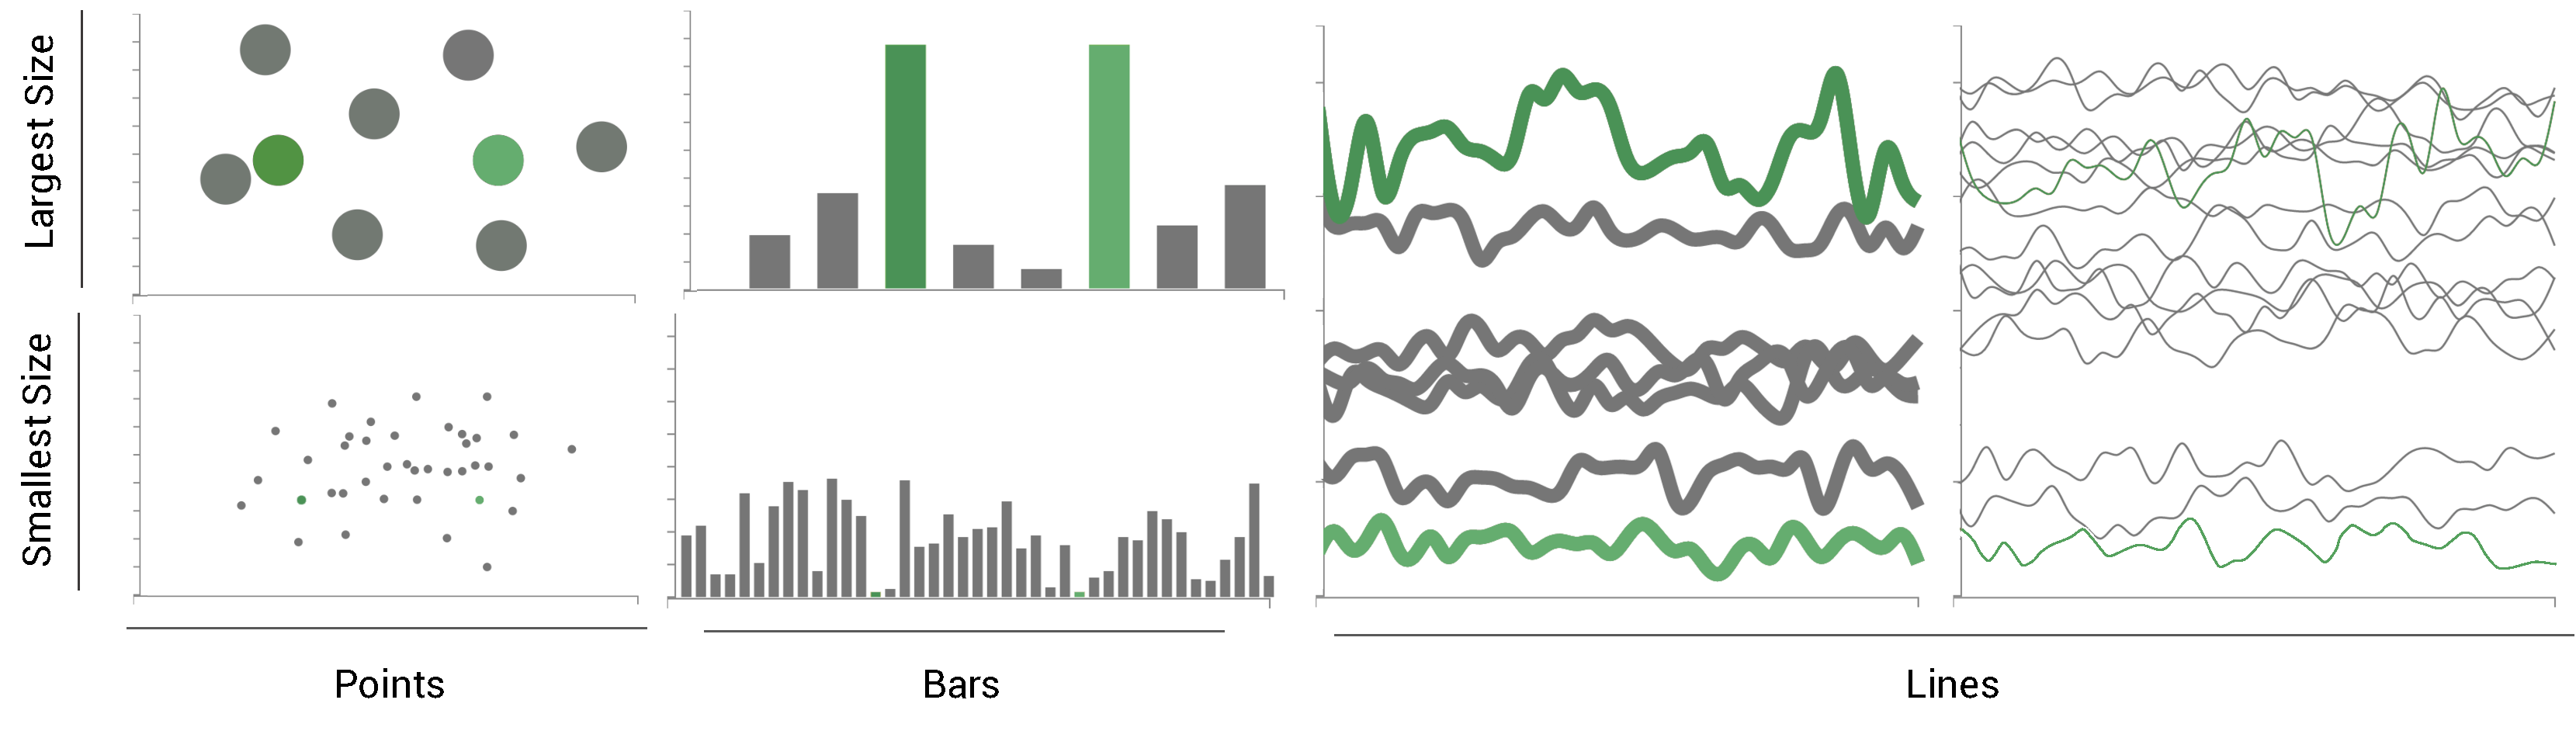
\includegraphics[width=0.48\textwidth]{teaserOne.pdf}
	\end{center}
	\caption{I build quantitative modeling of how people interpret data in different visualizations, blending vision, cognitive, and data science to encourage more effective design.}
\end{wrapfigure}

Color is commonly used to encode data; however, traditional color perception models underestimate people's abilities to distinguish data by a favor of five. This underestimation means people may be unable to disambiguate a significant proportion of their data. I construct quantitative models of visual perception specifically tailored to visualization to correct for these issues. Unlike conventional visualization studies, my research moves beyond A/B testing to generate actionable probabilistic models of data interpretation to guide effective visualization design. I received an NSF CRII (\$174,925) to support this research. The grant is intended to support the development of computational models of color perception in visualizations and the construction of an assistive color encoding design tool that blends these models with statistical models of expert design practices drawn from a corpus of encodings drawn from handcrafted encodings used in existing tools.
%Models developed during my Ph.D. provide significant improvements over conventional approaches, improving color disambiguation from 43\% to 99.8\% accuracy \cite{albers2014Designing}. 
Models developed in my 2017 IEEE VIS paper \cite{szafir2018Modeling} (Fig. \ref{color}) present data-driven quantitative models that optimize conventional color spaces for archetypal visualizations, such as scatterplots and bar charts. These models provide the first set of color perception models directly grounded in visualization practice. This research has been integrated into leading visualization tools, including Tableau and D3, and received the Best InfoVis Paper award at IEEE VIS, the flagship conference for visualization (top paper of 170 submissions). A Ph.D. student and two M.S. students have three papers in progress extending these models to capture the influence of size and shape on color perceptions in scatterplots and to develop the underlying algorithm and tool for assistive encoding generation, targeting CHI 2019 and IEEE VIS 2019 respectively. 
% InfoVis Best Paper Award, selected as the top paper out of 170 submissions, and was the first solo-authored paper to receive the award in over a decade. The resulting model was adapted into the design of Tableau 10. 

Additionally, I investigate how people synthesize information across large datasets, a process known as \emph{visual aggregation}. 
%As the amount of data available and the questions asked of that data continue to grow, visualizations must accommodate analyses across multiple datapoints simultaneously. However, 
Conventional understandings of how to encode data capture comparisons between two datapoints; however, growing datasets often require analysts to synthesize information from large numbers of datapoints simultaneously, such as averages, variance, or trends. My research was the first to introduce ideas from \emph{ensemble coding}--people's abilities to visually estimate statistical information--to predict how visualizations might support tasks involving multiple datapoints. 
%My work has explored the idea of \emph{visual aggregation} to the creation of visualizations to remedy this knowledge gap. By integrating information about the visual system's capacity to rapidly compute statistical information about a visual scene, I modeled how the visual representations that best supported statistical tasks synthesizing information across multiple datapoints, focusing on standard aggregate statistics, such as mean and variance. 
In this work, I demonstrated a fundamental tension between how well visualizations support comparisons at various scales. Visualizations well-suited for comparing individual values perform poorly for tasks requiring people to synthesize information across multiple datapoints, while those well-suited to this synthesis perform poorly for tasks involving individual values. 
%These observations led to two novel systems: \emph{Sequence Surveyor}, a system for genetic analyses, and \emph{TextDNA}, a system for literary analysis. These systems increased the scales of data that domain experts could analyze by an order of magnitude over previous approaches. 
%I built on these findings to introduce an interdisciplinary research agenda for visualization perceptions in the era of big data.
%in the Journal of Vision. 
I extended this work by developing a framework that reveals how fundamental principles from visual perception can predict the types of statistical information people extract from different visualizations. This framework introduced a new interdisciplinary research area that bridges computer and cognitive science and has become the fifth highest scoring Journal of Vision paper ever published according to Altmetric (in the top 5\% of all scored publications) \cite{szafir2016Four}. This research initiated a dialog with psychologists from Northwestern University, the University of British Columbia, and MIT have led to the founding of VisXVision, an organization of researchers aimed at encouraging collaborations between visualization researchers and vision scientists. We have successfully organized and hosted a panel at IEEE VIS and a symposium at the Vision Sciences Society Annual Meeting focusing on increasing the research dialog between these communities. Both events have attracted hundreds of researchers and have led to initial collaborations between my lab and researchers at the University of Wisconsin, Carleton College, and MIT. I have additionally started projects looking at visualization design and prediction in time series data and empirical data generation (led to a UROP for the student researcher) in this line of research. 

Given the substantial recent advances in analytic algorithms, I have extended my research in perceptual methods to consider cognitive aspects of design, especially for situations combining human and algorithmic analysis. These studies focus on the role of visualization and interaction on trust in data. The first of these studies arose from a collaboration with Prof. Michael Paul's group constructing a tool for iterative topic model refinement with fused CDC and social media data building on observations from \cite{pruss2018Zika}. Social media data often requires analysts work with missing or corrupted data due to failures in the data collection pipeline. With a M.S. student (beginning her Ph.D. at Georgia Tech in Fall 2018), we evaluate the role of different visualization designs and methods for estimating missing values on perceived data quality, focusing on confidence, credibility, reliability, and completeness in addition to estimation accuracy \cite{song2019Wheres}. This study presents the most comprehensive evaluation of design methods for missing data to date. We found a systematic relationship between the visual structure of the resulting representation: methods that break the visual continuity of data lead to lower perceived quality and even bias in estimation. This work has been conditionally accepted to IEEE VIS 2018. 

We extended these approaches to understand perceived trust in classification for collaborative human-machine classification in collaboration with Prof. Nisar Ahmed, a Ph.D. student, and an undergraduate (beginning his M.S. at CU in Fall 2018) \cite{iuzzolino2019In}. In this study, we asked people to help ``train'' a classifier to distinguish between different dog breeds by presenting them with a series of images and visualizations of the classifier's current confidence in the predicted breed. We presented people with one of eight common visualization approaches and asked them to label images according to six policies (e.g., all low-confidence images, a common approach maximizing the machine's information gain; all high-confidence images, theoretically maximizing human perceptions of performance; random low- and high-confidence images, etc.). Our results suggest that current approaches to integrating people into classifier training lead to significantly lower subjective and objective trust in outputs of a machine learning algorithm, up to a 2x increase in the number of disagreements for machine-oriented learning policies. The manuscript for this study is currently in revision for submission to CHI 2019. 

%Further, the interpretation of information doesn't stop with our sense of sight
%\todo[inline]{Cognitive Factors: Hayeong's study, Michael's study}

%\textbf{On-Going \& Future Work: }My current NSF-sponsored research integrates perceptual models with quantified models of heuristic best practices for data encoding. These heuristics describe how people select sets of colors to optimally represent data and are critical to effective visualization. However, it takes significant design expertise to use them effectively. I am creating statistical models of color encoding structure from a set of designer color maps used in visualizations to quantify these heuristics. 
%. I will model the design structure in expert-crafted encodings and blend these models with my previous perceptual models to generate a statistical model of effective color encoding. 
%integrate these models with data extracted from designer encodings to guide visualizations that adhere to both perceptual and expert designer practices. 
%I will combine the heuristic and perceptual models in an assistive design tool that allows people to rapidly construct visualizations that are grounded in perceptual science and best practices for visualizing data, reducing barriers to creating effective visualizations.

%Building on this framework, I am currently investigating the role of ensemble coding in decision making and visual data fusion. This work is measuring how visualizations can support analysts in prediction and fusion from multiple data sources across a range of domains, including defense and public health. %\vspace{-2pt}

%Interpretation of model parameters for data-driven reasoning about recommendations in QIMs

\emph{Student Advisees: }H. Bansal, M. Iuzzolino, C. Mcguinness, R. Mustari, S. Naidu, P. Sherkane, H. Song, S. Smart, T. Umada, K. Wu\\
\emph{Funding Sources:} National Science Foundation\\
% (\$174,925)
\emph{Publication Venues:} IEEE VIS (Best Paper Award), Journal of Vision, Vision Sciences Society

\textbf{T2--Scalable Visualization Systems: }
While Thread 1 allows us to understand how people interpret data in visualizations, Thread 2 focuses on how we can transfer this knowledge into systems that support data analysis for real-world problems. My work during my Ph.D. led to systems in genomics \cite{albers2014Sequence}, biochemistry \cite{sarikaya2014Molecular}, and literary analysis \cite{szafir2016TextDNA} that supported interactive exploration at scales an order of magnitude larger than prior approaches. My publication record in this thread is not as deep as others. Systems design, development, and deployment requires substantial time, especially when using the iterative user-centered design process I employ in my research. However, in addition to the above work, I have two systems projects currently underway with domain collaborators targeting submission within the near term. 

\begin{wrapfigure}{l}{0.5\textwidth}
	\begin{center}
		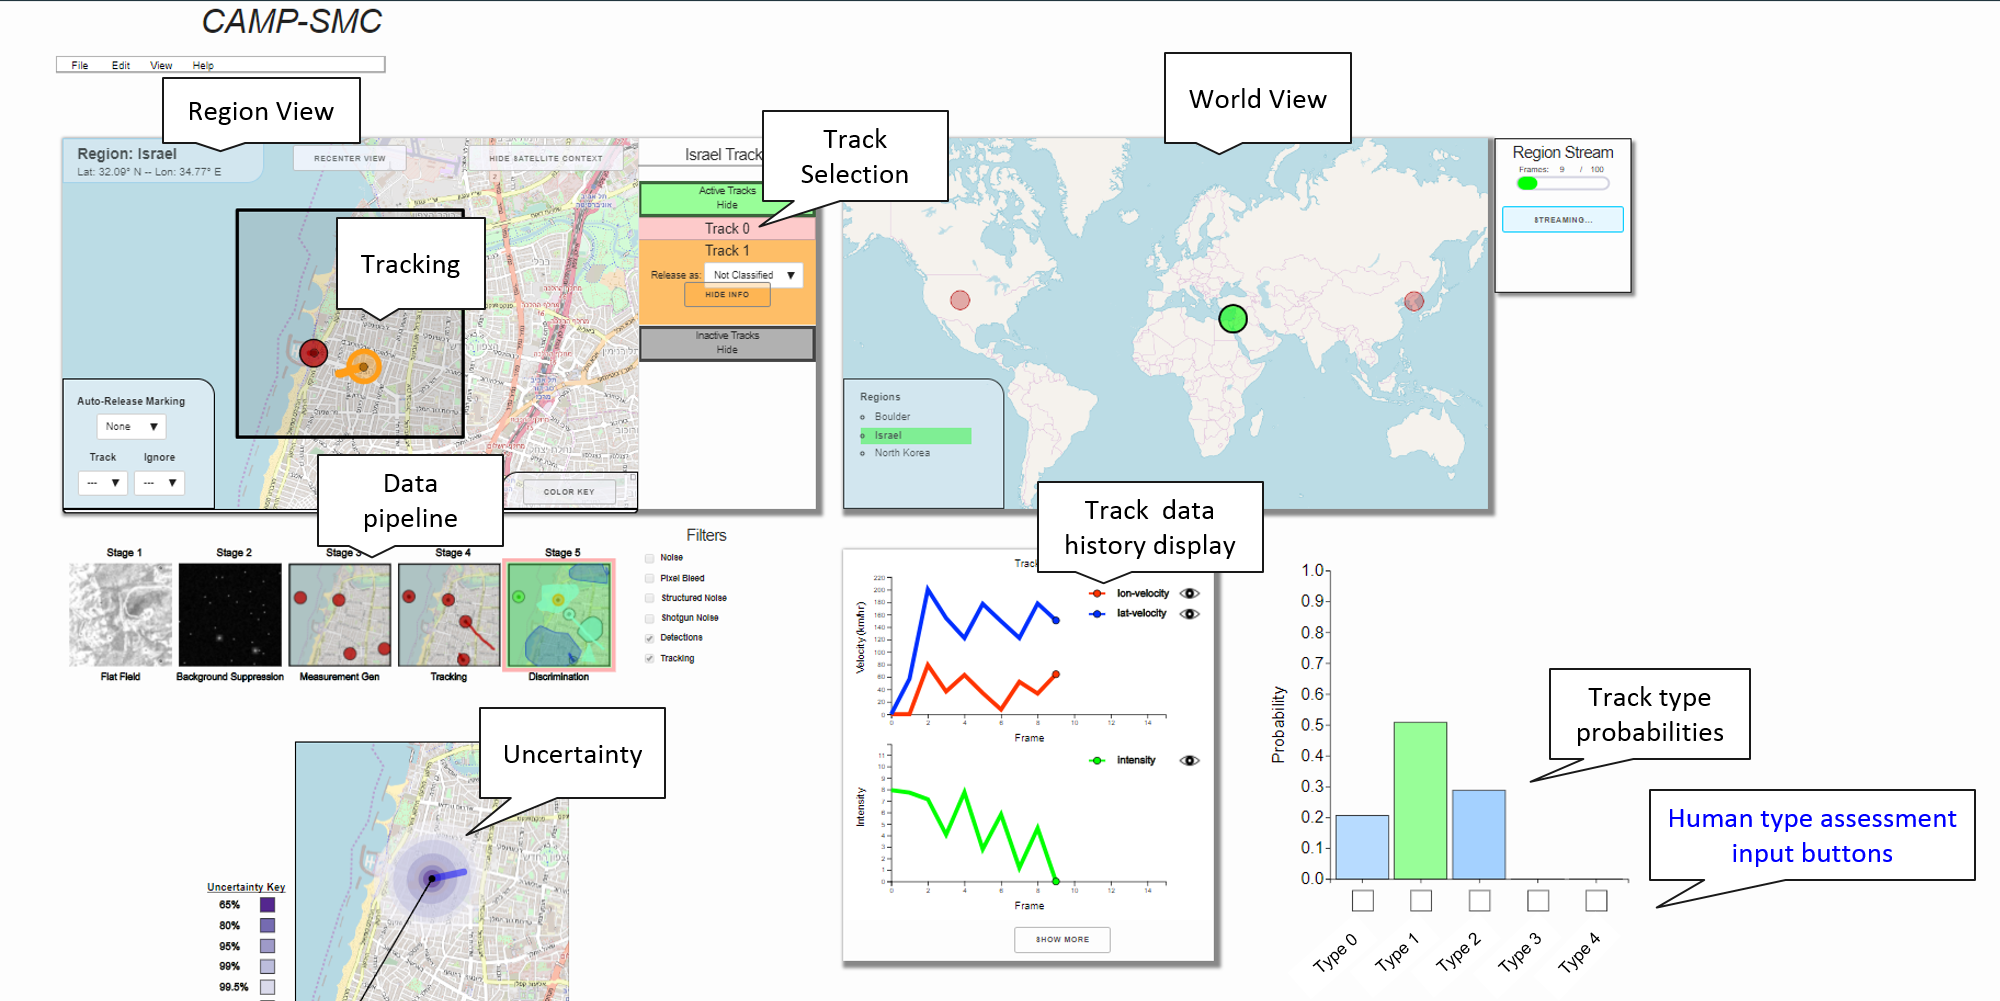
\includegraphics[width=0.48\textwidth]{interface}
	\end{center}
	\caption{The findings from our basic science work inform systems for collaborative human-machine analysis of large data, such as the CAMP system that enables intelligence analysts to rapidly detect and characterize threats in large-scale image data.}
\end{wrapfigure}

One line of research in this thread investigates how visualizations can support collaborative data exploration between people and automated processes. Although machine learning and related techniques are enabling analysts to process unprecedented quantities of data, such automation can obscure information about how data is processed and prevent analysts from applying their own contextual understandings, past experience, and domain expertise. I received a \$353,936 grant from the US Air Force in collaboration with Prof. Nisar Ahmed (data fusion expert) and Lockheed Martin to construct a system for collaborative human-in-the-loop analysis of OPIR satellite imaging data. Under this funding, we have developed the CAMP (collaborative analyst-machine perception, Fig. \ref{interface}) system, a visualization system for allowing military defense analysts to identify and characterize potential threats in large scale streaming collections of satellite images by combining visualization, computer vision, and machine learning. The system leverages backend data fusion algorithms designed by Prof. Ahmed's group with a novel interactive front-end developed by my lab and a human-in-the-loop integration of interactive feedback developed in collaboration between both labs \cite{muesing2019}. In simulation, our approach will likely accelerate time-to-detection and characterization in real-time datasets by 3 minutes and allow analysts to operate across large collections of image streams rather than the single stream monitoring process currently in use. The project has been recommended for additional funding to expand on the current research efforts and integrate the system into the Operational Battlespace Awareness Center for use in actual defense applications. 

In collaboration with a M.S. student and Prof. Michael Paul and Prof. Eric Alexander of Carleton College, we have additionally begun development of an interactive human-in-the-loop system for public health analysis. The system fuses data from the CDC (high quality, low throughput) and from social media (low quality, high throughput) to provide more holistic and scalable analysis of public health data. The core of the system pairs CDC data with social media to provide a quality check and contextualization for rapid disease survaillence and prediction. Further, to provide access to the underlying information and disease dissemination borrow from collaborations with Prof. Paul's lab \cite{pruss2019Zika}, we are developing an interactive visual analytics system based on sentiment analysis and topic modeling to extract common themes in social media data related to certain time or geographic points in order to access the underlying raw information and refine the themes and/or data interactively to mitigate quality concerns and integrate expert knowledge into decision making. The system is targeted for submission to IEEE VIS 2019.

In collaboration with Profs. Jed Brubaker, Casey Fiesler, and Michael Paul, I have started to explore how visualization systems might support scalable qualitative inductive methods (QIMs) for analyzing large text corpora. Current QIMs require deep manual processing of the data, integrating context and expertise for high-quality analysis, but limiting the proportion of a corpus to be analyzed and reproducibility of these analyses. The goal of this project, which has been recommended for funding by the NSF (\$1.1M), is to leverage machine learning, natural language processing, and transparency through interactive visualization and human-in-the-loop refinement to model human QIM application in text and recommend interesting passages for analysis. The algorithm observes expert analysis and steadily generates a model of different characterizations applied to text. The system will then provide recommendation of interesting passages for analysis as well as in-line visualizations of why the passage may be of interest and interactive refinement methods for dismissing and refining recommendations. The system will also allow analysts freeform exploration of label distributions and composition to allow for multiscale application of QIMs to generate classifiers that best capture expert interpretation for scalable expert-driven navigation of large corpora and analysis reproducability and explainability. Preliminary algorithmic development by my lab in collaboration with Prof. Brubaker's lab demonstrate that these methods can capture QIM outputs with reasonable accuracy even using basic algorithms. 

In addition to concrete systems work, I have begun exploring how visualizations might assemble a generalizable design framework for dealing with scalability issues. In \cite{sarikayadesign}, we present a systematic qualitative survey of how visualizations summarize large datasets and patterns in these techniques for different data types, tasks, and goals. This work is co-authored by my Ph.D. advisor as the lead student author was still working under his supervision at the time. However, I served as the primary faculty supervisor and technical lead on the research. We distilled patterns in use and design in XXX\todo{number} systems from the visualization literature. Through this distillation, we created an initial design space to help identify current trends and open opportunities for scalable visualization designs. This paper appeared at EuroVis 2018. 

% when the amount of data far exceeds the number of available pixels. 
%While visualizations can support large-scale analyses, the number of available pixels limits the exploratory capabilities of visualization systems. Statistical analyses overcome this limitation by computationally reducing the amount of data analysts explore. However, 
%Automated data processing scales well, but hides how the reduced data was generated. This obscuration prevents analysts from applying their own understanding to the analysis problem. 
%I use visualization to enable people and machines to \emph{collaboratively} analyze data, allowing people to focus on specific patterns in the data while automation rapidly mines these patterns at scale. For example, I designed a system for computational biochemists that improved protein binding site prediction. This system paired classification algorithms with task-oriented visualizations of prediction performance, aiding analysts in rapidly identifying patterns of interest over hundreds of molecular structures
%. On-demand surface visualizations contextualized predictions and empower biochemists to 
%and interactively reparameterizing algorithms to account for prediction biases. Through a grant from the U.S. Air Force, my current research explores how visualization can enable collaborative analysis of large spatiotemporal satellite image data. I am developing a system that automatically identifies important objects and behaviors based on historical data and provides interactive mapping and metadata visualizations that describe the features and uncertainties associated with the detection. 
%Analysts interact with detailed map overlays and feature-based visualizations to provide feedback on interesting objects and behavior to the detection algorithms. 
%This research is scaffolding the development of innovative applications in drought and wildfire monitoring by facilitating seamless analysis of key anomalies in satellite imagery fused with geospatial environmental data. %\vspace{-2pt}
%\todo[inline]{OBAC Launch}

%\todo[inline]{QIMs, Public Health Analyses, Continued model-driven reasoning, Design for accessible communities}

\emph{Student Advisees: } W. Braun, P. Deveraj, I. Fawaz, M. Iuzzolino, Y. Mahadasu, S. Nath, S. Prabhu, G. Ramkumar, H. Song, T. Umada, M. Xiao\\
\emph{Funding Sources:} National Science Foundation, US Air Force SMC-RSX\\
%National Science Foundation (\$1,070,508), US Air Force SMC-RSX (\$353,936)\\
\emph{Publication Venues:} EuroVis, AIAA@InfoTech (under review)

\textbf{T3--Embedded Analytics: }
Building on the HCI strengths at CU has additionally allowed me to expand my research focus to consider the role of context and situational awareness in data analysis. In particular, my research has begun to explore how augmented reality (AR) might enable interactively visualizations to directly bind data representations with the physical contexts those data represent. Because research in such immersive analytics is quite nascent, my work in this area has explored contextualized AR visualization at multiple levels, ranging from perception to interaction to full system design with stakeholders in environmental science and emergency response. 

In collaboration with Prof. Dan Szafir, one M.S. student, and one undergraduate who served as the student lead, we conducted a controlled laboratory study exploring how the different rendering techniques used in AR might change people's perceptions of where virtual objects are located in space \cite{diaz2017Designing}. By understanding which techniques allow people to best locate virtual objects in the physical world, we can tightly bind visualized data to its corresponding physical context. In a pair of studies evaluating eight \todo{check this} common graphics techniques conventionally correlated with spatial perceptions, we found that most conventional cues for spatial positioning had minimal effects on an object's perceived position and that synthetic stylized shadows supported more accurate and subjectively easier object localization in real-world scenes. This study, published at ISMAR 2017 (the premiere conference for augmented reality research), suggests that computationally expensive precise rendering and artificial integration of many spatial cues (e.g., texture and lighting) are unnecessary for data localization in modern AR head-mounted displays. 

\begin{wrapfigure}{l}{0.5\textwidth}
	\begin{center}
		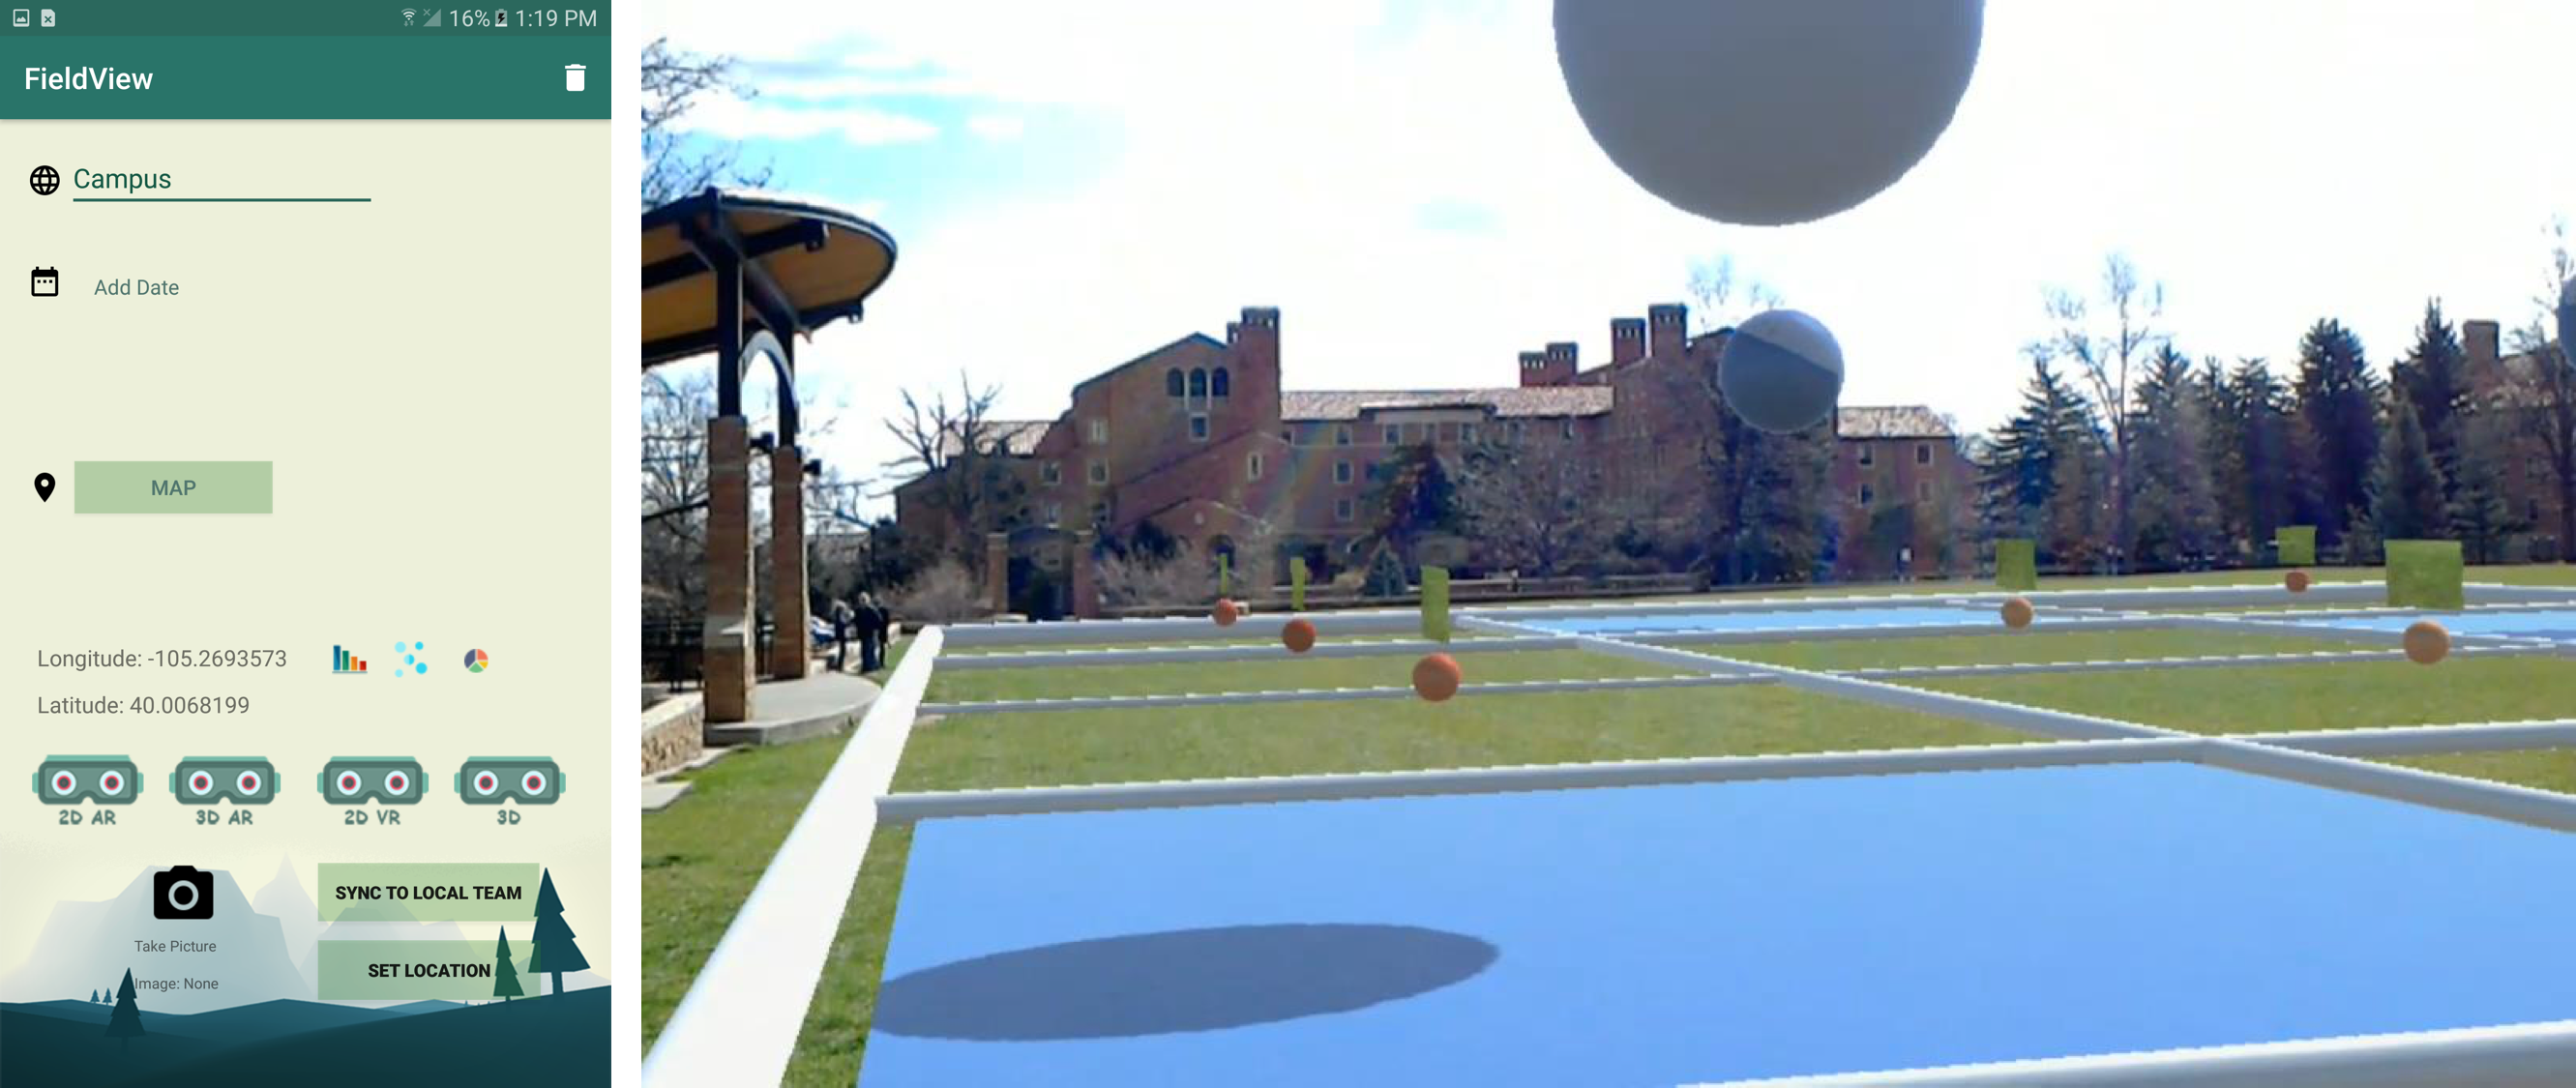
\includegraphics[width=0.48\textwidth]{fieldview}
	\end{center}
	\caption{By understanding the perceptual, cognitive, and interactive properties of immersive data analytics, we can design systems that allow analysts to capture and analyze data in real-time using mobile, cloud, and augmented reality technologies to bridge temporal and spatial gaps in field data use.}
\end{wrapfigure}
 
Embedding data in immersive environments may place data well beyond arm's reach. However, little is known about how to effectively engage with that data in interactive systems. To remedy this gap, I conducted a study in collaboration with two Ph.D. students and Profs. Shaun Kane and Jed Brubaker to empirically model preferred methods for interacting with distant data in AR \cite{whitlock2018Distal}. In this study, participants interacted with data from different Internet of Things devices at 8, 12, and 16 feet using controllers, voice, and gesture inputs. We collected objective (time to completion and task accuracy) and subjective (usability, preference, and perceived performance) data to compare the different modalities and determined that, while gesture inputs were significantly preferred overall, controller inputs performed as well or better than gesture inputs in all cases, while voice-based interactions were unsuitable for the tested tasks. The paper was presented at IEEE VR 2018, the premiere conference for virtual reality research. 

In collaboration with a Ph.D. student and two M.S. students, I used the outputs from the above studies to inform the design of an interactive system for exploring field-collected data \cite{whitlock2018FieldView}. Funded by a CU Innovative Seed Grant (\$30,000), we conducted a series of interviews with environmental scientists, field roboticists, climate scientists, and emergency responders to understand the limitations of field data analysis under current practices. These discussions identified critical gaps in time and context that limited data use, quality, collaboration, and collection practices with current technologies. We constructed a prototype system using a mobile phone application for data collection and basic visualization coupled with a cloud datastore and immersive visualization to support in-the-field data analysis. We then used this system as a design prompt to collect feedback on how the technology might enhance field data use and collection with 10 experts. \todo{check number} From these interviews, we refined our system to enable situated data collection and analysis to improve data quality, collaborative practice, and situated analysis in the field, empower field researchers to improve their data use and decision making while in the field (Fig. \ref{fieldview}). The paper for this system is currently under review for UIST 2018, a top-tier conference on user interface technologies. 

In collaboration with Profs. Dan Szafir and Christoffer Heckman, I am serving as the Co-PI on a recommended NSF grant (\$1.2M) to use the principles introduced in FieldView to design a system for improved integration of data from both human partners and sensing devices such as robots for rapid decision making in emergency response scenarios. In this proposal, my team will conduct a quantitative evaluation of how the visual affordances of AR, including stereoviewing and physical context, change the effectiveness of common visualization types. Using this data paired with interviews with emergency response teams, we will develop a novel visualization system for situated analysis targeted directly at emergency responders operating in the field. The goal of this system is to empower and enrich data-driven decision making in the field to improve emergency response practices under changing environments. 

%NSF Grant
In addition to this work, I have two early-phase student-led projects exploring AR in other contexts. The first is exploring how interactive visualizations can be overlaid on physicalizations of data. The goal of this project is to leverage interactive AR to support collaborative data exploration between sighted and non-sighted users. The second project is an interactive system for in-situ prototyping. In collaboration with a Ph.D. student and an undergraduate senior capstone team, the MR-CAT system allows for situated content authoring in augmented reality, reducing barriers to environment-scale AR application development. We are currently in-process of refining the application for museum settings based on discussions with target stakeholders to support rapid prototyping of interactive AR exhibits and with Ball Aerospace for applying the prototyping solution to engineering applications including product refinement and training. 
%Justin's stuff, Ball Aerospace

\todo[inline]{integrate images throughout}

\emph{Student Advisees:} J. Chin, M. Natarjan, A. Thompson, M. Whitlock, K. Wu, MR-CAT Team\\
\emph{Funding Sources:} National Science Foundation, CU Innovative Seed Grant Program\\
%National Science Foundation (\$1,194,056), Innovative Seed Grant Program (\$30,000)  \\
\emph{Publication Venues:} IEEE VR, ACM/IEEE ISMAR, ACM UIST (under review)

\section*{Career Research Trajectory}

My overall research agenda aims to understand how we can leverage visualization to make exploratory data analysis more accurate, scalable, and holistic. I achieve this by modeling how people interpret visualizations, using this understanding to drive novel analytic systems, and integrating novel technologies into visualization approaches in order to overcome contextual barriers to analysis. My work at CU has resulted in seven top-tier conference and journal publications, over \$2M in funding from national agencies, and research mentorship of 23 students. 

Through the on-going and up-coming projects listed above, my near-term research agenda will focus more deeply on system development. Recent funding successes afford the opportunity to shift more of my scholarly writing time to research support and expanded collaboration with researchers external to CU with which discussions have already begun for preliminary steps towards publishable interdisciplinary projects. To support this work, I intend to focus additional efforts towards recruiting additional Ph.D. students through funded RAships in Information Science.  
%Future trajectory: Focus more on system development, slowing grant writing and focusing on production in the near term. 
%Target Impact: make data science more accessible through empirical, user-centered approaches. Benefits both designers and users
My goal through this research is to advance the field of data science by developing tools, guidelines, models, and methods that empower people, allowing them to drive analyses through interactive systems that support reliable and meaningful use of data.
%In my research and my work as founding faculty in the new Department of Information Science at CU Boulder, I aim to advance the field of data science by developing tools and methods that empower people, allowing them to drive analyses through interactive systems that support reliable and meaningful use of data. 


{
\vspace{4pt}
\noindent
\textbf{References}
\vspace{-36pt}
\renewcommand\refname{\vskip -1cm}
\small
\bibliographystyle{abbrv}
\bibliography{main}
}


\pagebreak
\setcounter{page}{1}


\end{document}
